\documentclass[12pt]{article}
\usepackage[utf8]{inputenc}
\usepackage[dvips]{graphicx}
\usepackage{fancybox}
\usepackage{verbatim}
\usepackage{multirow,array}
\usepackage{latexsym}
\usepackage{alltt}
\usepackage{hyperref}
\usepackage{textcomp}
\usepackage{color}
\usepackage{amsmath}
\usepackage{amsfonts}
\usepackage{tikz}
\usepackage{float}
\usepackage{amssymb}
\usepackage{multicol}
\usepackage[shortlabels]{enumitem}

\usepackage[hmargin=3cm,vmargin=6.0cm]{geometry}
%\topmargin=0cm
\topmargin=-2cm
\addtolength{\textheight}{6.5cm}
\addtolength{\textwidth}{2.0cm}
%\setlength{\leftmargin}{-5cm}
\setlength{\oddsidemargin}{0.0cm}
\setlength{\evensidemargin}{0.0cm}

\begin{document}

\section*{Student Information } 
%Write your full name and id number between the colon and newline
%Put one empty space character after colon and before newline
Full Name : Doruk Berke Yurtsızoğlu  \\
Id Number : 2522225 \\

% Write your answers below the section tags
\section*{Answer 1}
At first, let's say $$F(x) = \sum^{\infty}_{n=0} F_n \cdot x^n$$\\
\\
We know that recursion relation that was given in the question is applicable when $n \geq 2$. Then, if we want to represent the recursion relation with using sigma notation, it will look like:\\
\\
$ \sum^{\infty}_{n=2} F_n \cdot x^n = 3 \cdot  \sum^{\infty}_{n=2} F_{n-1} \cdot x^n + 4 \cdot \sum^{\infty}_{n=2} F_{n-2} \cdot x^n$\\
\\
We know that $F(x) = \sum^{\infty}_{n=0} F_n \cdot x^n$, then we can write the expressions above as:\\
\\
$ \sum^{\infty}_{n=2} F_n \cdot x^n = F(x) - a_0 - a_1 \cdot x = F(x) -1 - x$ (since $a_0 = 1\ and\ a_1 =1)$\\
\\
$3 \cdot \sum^{\infty}_{n=2}  F_{n-1} \cdot x^n = 3x \cdot \sum^{\infty}_{n=2}  F_{n-1} \cdot x^{n-1} =  3x \cdot (F(x) - a_0)$\\
\\
$4 \cdot \sum^{\infty}_{n=2}  F_{n-2} \cdot x^n = 4x^2 \cdot \sum^{\infty}_{n=2}  F_{n-2} \cdot x^{n-2} =  4x^2 \cdot F(x)$\\
\\
From the sigma notation representations and the recursion relation, we get an equation that i the form of:\\
$F(x) -1 - x =  3x \cdot (F(x) - a_0) + 4x^2 \cdot F(x)$\\
$F(x) - 3x \cdot F(x) - 4x^2 \cdot F(x) = 1 -2x $\\
$F(x) \cdot (1 - 3x -4x^2) = 1 - 2x$\\
\\
We ended up with the equation $F(x) = \dfrac{1 - 2x}{1 - 3x - 4x^2} = \dfrac{2x - 1}{4x^2 + 3x -1}$\\
\\
We can simplify the equation by using partial fraction method.\\
$F(x) = \dfrac{2x - 1}{4x^2 + 3x -1} = \dfrac{A}{4x-1} + \dfrac{B}{x+1}$\\
\\
Now, we are going to solve the equation:\\
$Ax + A + 4Bx -B = 2x -1$\\
$A + 4B = 2$, $A-B = -1$\\
$A = \dfrac{-2}{5}$ and $B = \dfrac{3}{5}$\\
\\
After applying these steps, our equation transformed into the form:\\
\\
$F(x) = \dfrac{2x - 1}{4x^2 + 3x -1} = \dfrac{1}{5} \cdot (\dfrac{2}{1-4x} + \dfrac{3}{1+x})$\\
\\
Now, we are going to use the information $\dfrac{1}{1-ax} = \sum^{\infty}_{k=0} a^k \cdot x^k$ and implement it to our equation.\\
$\dfrac{2}{5} \cdot \dfrac{1}{4x-1} = \dfrac{2}{5} \cdot \sum^{\infty}_{n=0} 4^n \cdot x^n$\\
\\
$\dfrac{3}{5} \cdot \dfrac{1}{1+x} = \dfrac{3}{5} \cdot \sum^{\infty}_{n=0} (-1)^n \cdot x^n$\\
\\
If we sum up these two equations, we will get $\sum^{\infty}_{n=0} \dfrac{2}{5} \cdot 4^n \cdot x^n + \dfrac{3}{5} \cdot (-1)^n \cdot x^n$ \\
Which is equal to $\sum^{\infty}_{n=0} \dfrac{2 \cdot 2^2n + 3\cdot(-1)^n}{5} \cdot x^n$\\
\\
In conclusion, we know that $F(x) = \sum^{\infty}_{n=0} F_n \cdot x^n$ from the beginning of the solution. Also, we get an equation that represents $F(x)$ as  $\sum^{\infty}_{n=0} \dfrac{2 \cdot 2^2n + 3\cdot(-1)^n}{5} \cdot x^n$\\
\\
Then, by combining these two equation, we can conclude that \\
\\
$a_n = \dfrac{2 \cdot 2^2n + 3\cdot(-1)^n}{5} = \dfrac{1}{5} \cdot (2^{2n + 1} + 3\cdot (-1)^n)$\\



\section*{Answer 2}
\subsection*{a) }
Power series representation of the sequence will be:\\
$A(x) = 2 + 5x + 11x^2 + 29x^3 + 83x^4 + 245x^5 ...$ (where A(x) is the generative function of the sequence)\\
$= (2 + 2x + 2x^2 + 2x^3 +2x^4 + ...) + (3x + 9x^2 + 27x^3 + 81x^4 + ...)$\\
$= 2(1 + x + x^2 + x^3 + x^4 + ...) + 3x(1 + 3x + 9x^2 + 27x^2 + ...)$\\
\\
We will use the information, $1 + x + x^2 + x^3 + x^4 + ... = \sum^{\infty}_{n=0} x^n = \dfrac{1}{1-x}$\\
\\
$2(1 + x + x^2 + x^3 + x^4 + ...) = 2 \cdot \sum^{\infty}_{n=0} x^n = \dfrac{2}{1-x}$\\
\\
$3x(1 + 3x + 9x^2 + 27x^2 + ...) = \sum^{\infty}_{n=0} 3^n \cdot x^n = \dfrac{3x}{1-3x}$\\
\\
The equations we know:\\
$-$$A(x) = 2(1 + x + x^2 + x^3 + x^4 + ...) + 3x(1 + 3x + 9x^2 + 27x^2 + ...)$\\
\\
$-$$2(1 + x + x^2 + x^3 + x^4 + ...) = \dfrac{2}{1-x}$\\
\\
$-$$3x(1 + 3x + 9x^2 + 27x^2 + ...) = \dfrac{3x}{1-3x}$\\
\\
Then, we can conclude that, $A(x) = \dfrac{2}{1-x} + \dfrac{3x}{1-3x} = \dfrac{-3x^2 - 3x + 2}{3x^2 - 4x + 1}$ is the generative function of the sequence.\\


\subsection*{b) }

$G(x) =\dfrac{7-9x}{1-3x+2x^2}$, $1-3x+2x^2 = (1-2x)\cdot(1-x)$ so we can use partial fractions method.\\ 
\\
$\dfrac{7-9x}{1-3x+2x^2} = \dfrac{A}{1-2x} + \dfrac{B}{1-x}$\\
\\
$A - Ax - 2Bx + B = 7 - 9x$\\
$A + B = 7$ and $2A + B = 9$\\
$A = 5$, $B = 2$\\
\\
Then, $G(x) =\dfrac{7-9x}{1-3x+2x^2} = \dfrac{5}{1-2x} + \dfrac{2}{1-x}$\\
\\
$\dfrac{5}{1-2x} = 5 \cdot \sum^{\infty}_{n=0} 2^n x^n$\\
\\
$\dfrac{2}{1-x} = 2 \cdot \sum^{\infty}_{n=0} x^n$\\
\\
In conclusion, $G(x) =\dfrac{7-9x}{1-3x+2x^2} = \dfrac{5}{1-2x} + \dfrac{2}{1-x} = 5 \cdot \sum^{\infty}_{n=0} 2^n x^n + 2 \cdot \sum^{\infty}_{n=0} x^n$\\
\\
We know that, general generative function equation is $G(x) = \sum^{\infty}_{n=0} a_n \cdot x^n$\\
\\
Then, we will get the equation, $G(x) = \sum^{\infty}_{n=0} (5*2^n + 2) \cdot x^n = \sum^{\infty}_{n=0} a_n \cdot x^n$\\
\\
This means $a_n = 5*2^n + 2$\\

\section*{Answer 3}
\subsection*{a) }

The relation R represents the Pythagoras Theorem for positive natural numbers. So, the relation R states that aRb is true when both a and b are positive natural numbers and there exists a number n which is also a positive natural number and satisfies the the equations $n = \sqrt{a^2 + b^2}$ or $a = \sqrt{n^2 + b^2}$ or $b = \sqrt{a^2 + n^2}$.\\
\\Now, by using these informations, we are going to check if aRb is an eqivalence relation. A relation is an equivalence relation if it is reflexsive, symmetric and transitive. At first, we are going to look at the reflexsive property. A function is said to be reflexsive if we can construct a relation like aRa for all a. For our relation, aRa means  there exists a number n which satisfies the equations $n = \sqrt{a^2 + a^2}$ or $a = \sqrt{n^2 + a^2}$ or $a = \sqrt{a^2 + n^2}$.\\
For the first equation, since a is natural number, n will be $a\sqrt{2}$ which can't be a positive natural number in any cases.
For the second and third equations, the only way of satisfying these equations is taking $n = 0$ which can't happen since n must be a positive natural number.\\
So, we can conclude that the relation R is not an equivalence relation, since it doesn't satisfies the reflexive property.\\


\subsection*{b) }

We are going to check if the relation is reflexive, symmetric and transitive to decide if R is an equivalence relation.\\
\\
$-$Reflexive:\\
If the relation is reflexive it should satisfy $\implies$ $(x_1,y_1)R(x_1,y_1)$\\
$(x_1,y_1)R(x_1,y_1)$ gives us $2x_1 + y_1 = 2x_1 +y_1$. Thus, the relation R is reflexive.\\
\\
$-$Symmetric:\\
If the relation is symmetric, $(x_1,y_1)R(x_2,y_2) = (x_2,y_2)R(x_1,y_1)$ must be true.\\
$(x_1,y_1)R(x_2,y_2)$ gives us $2x_1 + y_1 = 2x_2 +y_2$ and $(x_2,y_2)R(x_1,y_1)$ gives us $2x_2 + y_2 = 2x_1 +y_1$. So, $(x_1,y_1)R(x_2,y_2) = (x_2,y_2)R(x_1,y_1).$Thus, the relation R is symmetric.\\
\\
$-$Transitive:\\
If the relation is transitive, $(x_1,y_1)R(x_2,y_2) = (x_2,y_2)R(x_3,y_3)$ then $(x_1,y_1)R(x_3,y_3)$ must be true.\\
$(x_1,y_1)R(x_2,y_2)$ gives us $2x_1 + y_1 = 2x_2 +y_2$ and $(x_2,y_2)R(x_3,y_3)$ gives us $2x_2 + y_2 = 2x_3 +y_3$. So, $2x_1 + y_1 = 2x_2 +y_2 = 2x_3 +y_3$.Thus, the relation R is transitive.\\
\\
Finally, we can conclude that the relation R is an equivalence relation.\\
\\
The equivalence class of $(1,-2)$ consists of all real pairs $(x,y)$ which satisfy $(x,y)R(1,-2)$. Then we will get $2*1 + (-2) = 2x + y = 0$\\
This equivalence relation represents the $2x + y = 0$ line in the Cartesian coordinate system.\\

\section*{Answer 4}
\subsection*{a) }

The unedited graph which consists of all connections is $(2,2), (5,5), (10,10), (18,18), (60,60), (2,60),\\ (5,10), (5,60), (2,10), (2,18), (10,60)$\\
\begin{figure}[H]
	\centering
	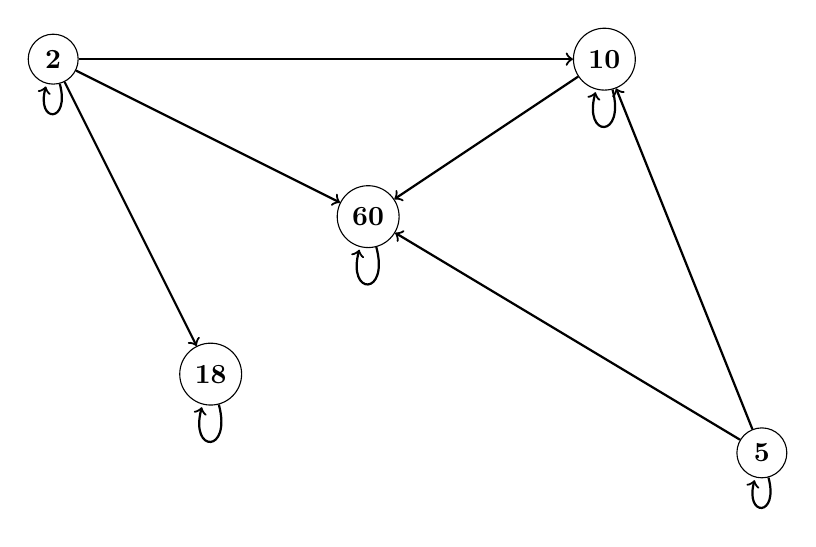
\begin{tikzpicture}
	
	\node[shape=circle,draw=black] (a) at (10, 5)    {\textbf{5}};
	
	
	\node[shape=circle,draw=black] (b) at (5, 8)   {\textbf{60}};
	\node[shape=circle,draw=black] (c) at (1, 10)   {\textbf{2}};
	
	
	\node[shape=circle,draw=black] (d) at (8, 10)   {\textbf{10}};
	
	\node[shape=circle,draw=black] (e) at (3, 6)    {\textbf{18}};

	\path[->, thick] (a) edge [loop below] (a);
	\path[->, thick] (b) edge [loop below] (b);
	\path[->, thick] (c) edge [loop below] (c);
	\path[->, thick] (d) edge [loop below] (d);
	\path[->, thick] (e) edge [loop below] (e);

	\path[->, thick] (a) edge (b);
	\path[->, thick] (a) edge (d);
	\path[->, thick] (c) edge (d);
	\path[->, thick] (c) edge (b);
	\path[->, thick] (c) edge (e);
	\path[->, thick] (d) edge (b);


\end{tikzpicture}
\end{figure}
Now, we are going to remove all loops and the connections that implied by the transitive property. The connections we will delete are $(2,2), (5,5), (10,10), (18,18), (60,60), (2,60), (5,60)$\\
\\
\begin{figure}[H]
	\centering
	\begin{tikzpicture}
	
	\node[shape=circle,draw=black] (a) at (8, 6)    {\textbf{5}};
	
	
	\node[shape=circle,draw=black] (b) at (6, 12)   {\textbf{60}};
	\node[shape=circle,draw=black] (c) at (4, 6)   {\textbf{2}};
	
	
	\node[shape=circle,draw=black] (d) at (6, 9)   {\textbf{10}};
	
	\node[shape=circle,draw=black] (e) at (2, 9)    {\textbf{18}};


	
	\path[->, thick] (a) edge (d);
	\path[->, thick] (c) edge (d);
	
	\path[->, thick] (c) edge (e);
	\path[->, thick] (d) edge (b);

	
\end{tikzpicture}
\caption{The Hasse Diagram}
\end{figure}


\subsection*{b) }
$-$Vertical axis is a, horizontal axis is b.\\
$-$Number 1 in the matrix tells us the element in the row of 1 divides the element in the column of 1.\\
$-$Number 1 in the matrix tells us the element in the row of 0 doesn't divide the element in the column of 0.\\
\\
The connections are $(2,2), (5,5), (10,10), (18,18), (60,60), (2,60), (5,10), (5,60), (2,10), (2,18), (10,60)$
\begin{figure}[H]
            $$  
                \begin{bmatrix}{}
                  &\vline 2 & 5 & 10 & 18 & 60 \\ 
			\hline
		  2 &\vline 1 & 0 & 1 & 1 & 1 \\
               5 &\vline 0 & 1 & 1 & 0 & 1 \\
              10 &\vline 0 & 0 & 1 & 0 & 1 \\
              18 &\vline 0 & 0 & 0 & 1 & 0 \\
		  60 &\vline 0 & 0 & 0 & 0 & 1 \\
                \end{bmatrix}{} 
            $$
		\caption{The Matrix Representation}
            \end{figure}{}

\subsection*{c) }
$R_s = R \cup ((b,a)|(a,b) \in R)$\\
$(2,2), (5,5), (10,10), (18,18), (60,60), (2,60), (5,10), (5,60), (2,10), (2,18), (10,60), (10, 2),(18, 2),\\(60, 2),(10, 5),(60, 5),(60, 10)$\\
\begin{figure}[H]
            $$  
                \begin{bmatrix}{}
                  &\vline 2 & 5 & 10 & 18 & 60 \\ 
			\hline
		  2 &\vline 1 & 0 & 1 & 1 & 1 \\
               5 &\vline 0 & 1 & 1 & 0 & 1 \\
              10 &\vline 1 & 1 & 1 & 0 & 1 \\
              18 &\vline 1 & 0 & 0 & 1 & 0 \\
		  60 &\vline 1 & 1 & 1 & 0 & 1 \\
                \end{bmatrix}{} 
            $$
		\caption{The Matrix Representation}
            \end{figure}{}

The list of (x,y) pairs in $R_s$ which is not present in R are:
$(10,2),(18,2),(60,2),(10,5),(60,5),(60,10)$\\
\subsection*{d) }
R is called totally ordered if every two elements of R are comparable. However, in our case, we can't compare $(2,5), (5,18), (10,18), (18,60)$.\\
If we look closely to the incomparable couples, we can see that both 5 and 18 has more than one incomparable elements which makes them the problematic elements.\\
By removing only one element, we can't get total order since we have two problematic elements. We have to delete both of them. After the deleting them both, if we are going to add an element and want to preserve the total order, we can choose the element from  (1, 20, 30, 120, 180...). Which are either divisor of 60 and multiple of 2 and 10 or multiple of 2, 10 and 60 or divisor of 2, 10, 60.\\
\\
For example if we remove both 5 and 18, then add 30 to the Hasse Diagram, the diagram will look like:\\
\\
\begin{figure}[H]
	\centering
	\begin{tikzpicture}
	
	
	\node[shape=circle,draw=black] (a) at (8, 13)   {\textbf{60}};
	\node[shape=circle,draw=black] (b) at (5, 4)   {\textbf{2}};
	
	
	\node[shape=circle,draw=black] (c) at (7, 7)   {\textbf{10}};
	\node[shape=circle,draw=black] (d) at (6, 10)   {\textbf{30}};
	


	
	%\path[->, thick] (a) edge (g);
	\path[->, thick] (b) edge (c);
	
	%\path[->, thick] (d) edge (h);
	\path[->, thick] (c) edge (d);
	\path[->, thick] (d) edge (a);


	
\end{tikzpicture}
\caption{The New Hasse Diagram Which Is In Total Order}
\end{figure}


\end{document}